\XtoCBlock{PILimit}
\label{block:PILimit}
\begin{figure}[H]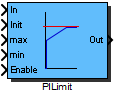
\includegraphics{PILimit}\end{figure} 

\begin{XtoCtabular}{Inports}
In & Control error input\tabularnewline
\hline
Init & Value which is loaded at initialization function call\tabularnewline
\hline
max & Maximum output value\tabularnewline
\hline
min & Minimum output value\tabularnewline
\hline
Enable & Enable == 0: Deactivation of block; Out set to 0

Enable 0->1: Preload of integral part

Enable == 1: Activation of block\tabularnewline
\hline
\end{XtoCtabular}


\begin{XtoCtabular}{Outports}
Out & \tabularnewline
\hline
\end{XtoCtabular}

\begin{XtoCtabular}{Mask Parameters}
Kp & Proportional Factor\tabularnewline
\hline
Ki & Integral Factor\tabularnewline
\hline
ts\_fact & Multiplication factor of base sampling time (in integer format)\tabularnewline
\hline
\end{XtoCtabular}

\subsubsection*{Description:}
PI controller with output limitation:

    G(s) = Kp + Ki/s

% include optional documentation file
\InputIfFileExists{\XcHomePath/Library/Control/Doc/PILimit_Info.tex}{\vspace{1ex}}{}

\subsubsection*{Implementations:}
\begin{tabular}{l l}
\textbf{FiP8} & 8 Bit Fixed Point Implementation\tabularnewline
\textbf{FiP16} & 16 Bit Fixed Point Implementation\tabularnewline
\textbf{FiP32} & 32 Bit Fixed Point Implementation\tabularnewline
\textbf{Float32} & 32 Bit Floating Point Implementation\tabularnewline
\textbf{Float64} & 64 Bit Floating Point Implementation\tabularnewline
\end{tabular}

\XtoCImplementation{FiP8}
\index{Block ID!3232}
\nopagebreak[0]
% Implementation details
\begin{tabular}{l l}
\textbf{Name} & FiP8 \tabularnewline
\textbf{ID} & 3232 \tabularnewline
\textbf{Revision} & 2.0 \tabularnewline
\textbf{C filename} & PILimit\_FiP8.c \tabularnewline
\textbf{H filename} & PILimit\_FiP8.h \tabularnewline
\end{tabular}
\vspace{1ex}

8 Bit Fixed Point Implementation

\begin{XtoCtabular}{Controller Parameters}
b0 & Integral coefficient\tabularnewline
\hline
b1 & Proportional coefficient\tabularnewline
\hline
sfrb0 & Shift factor for PI coefficient b0\tabularnewline
\hline
sfrb1 & Shift factor for PI coefficient b1\tabularnewline
\hline
i\_old & Integrator value of previous cycle\tabularnewline
\hline
enable\_old & Enable value of previous cycle\tabularnewline
\hline
\end{XtoCtabular}

% Implementation data structure
\XtoCDataStruct{Data Structure:}
\begin{lstlisting}
typedef struct {
     uint16        ID;
     int8          *In;
     int8          *Init;
     int8          *max;
     int8          *min;
     int8          *Enable;
     int8          Out;
     int8          b0;
     int8          b1;
     int8          sfrb0;
     int8          sfrb1;
     int16         i_old;
     int8          enable_old;
} PILIMIT_FIP8;
\end{lstlisting}

\ifdefined \AddTestReports
\InputIfFileExists{\XcHomePath/Library/Control/Doc/Test_PILimit_FiP8.tex}{}{}
\fi
\XtoCImplementation{FiP16}
\index{Block ID!3233}
\nopagebreak[0]
% Implementation details
\begin{tabular}{l l}
\textbf{Name} & FiP16 \tabularnewline
\textbf{ID} & 3233 \tabularnewline
\textbf{Revision} & 2.0 \tabularnewline
\textbf{C filename} & PILimit\_FiP16.c \tabularnewline
\textbf{H filename} & PILimit\_FiP16.h \tabularnewline
\end{tabular}
\vspace{1ex}

16 Bit Fixed Point Implementation

\begin{XtoCtabular}{Controller Parameters}
b0 & Integrall coefficient\tabularnewline
\hline
b1 & Proportional coefficient\tabularnewline
\hline
sfrb0 & Shift factor for PI coefficient b0\tabularnewline
\hline
sfrb1 & Shift factor for PI coefficient b1\tabularnewline
\hline
i\_old & Integrator value of previous cycle\tabularnewline
\hline
enable\_old & Enable value of previous cycle\tabularnewline
\hline
\end{XtoCtabular}

% Implementation data structure
\XtoCDataStruct{Data Structure:}
\begin{lstlisting}
typedef struct {
     uint16        ID;
     int16         *In;
     int16         *Init;
     int16         *max;
     int16         *min;
     int8          *Enable;
     int16         Out;
     int16         b0;
     int16         b1;
     int8          sfrb0;
     int8          sfrb1;
     int32         i_old;
     int8          enable_old;
} PILIMIT_FIP16;
\end{lstlisting}

\ifdefined \AddTestReports
\InputIfFileExists{\XcHomePath/Library/Control/Doc/Test_PILimit_FiP16.tex}{}{}
\fi
\XtoCImplementation{FiP32}
\index{Block ID!3234}
\nopagebreak[0]
% Implementation details
\begin{tabular}{l l}
\textbf{Name} & FiP32 \tabularnewline
\textbf{ID} & 3234 \tabularnewline
\textbf{Revision} & 2.0 \tabularnewline
\textbf{C filename} & PILimit\_FiP32.c \tabularnewline
\textbf{H filename} & PILimit\_FiP32.h \tabularnewline
\end{tabular}
\vspace{1ex}

32 Bit Fixed Point Implementation

\begin{XtoCtabular}{Controller Parameters}
b0 & Integrall coefficient\tabularnewline
\hline
b1 & Proportional coefficient\tabularnewline
\hline
sfrb0 & Shift factor for PI coefficient b0\tabularnewline
\hline
sfrb1 & Shift factor for PI coefficient b1\tabularnewline
\hline
i\_old & Integrator value of previous cycle\tabularnewline
\hline
enable\_old & Enable value of previous cycle\tabularnewline
\hline
\end{XtoCtabular}

% Implementation data structure
\XtoCDataStruct{Data Structure:}
\begin{lstlisting}
typedef struct {
     uint16        ID;
     int32         *In;
     int32         *Init;
     int32         *max;
     int32         *min;
     int8          *Enable;
     int32         Out;
     int32         b0;
     int32         b1;
     int8          sfrb0;
     int8          sfrb1;
     int64         i_old;
     int8          enable_old;
} PILIMIT_FIP32;
\end{lstlisting}

\ifdefined \AddTestReports
\InputIfFileExists{\XcHomePath/Library/Control/Doc/Test_PILimit_FiP32.tex}{}{}
\fi
\XtoCImplementation{Float32}
\index{Block ID!3235}
\nopagebreak[0]
% Implementation details
\begin{tabular}{l l}
\textbf{Name} & Float32 \tabularnewline
\textbf{ID} & 3235 \tabularnewline
\textbf{Revision} & 2.0 \tabularnewline
\textbf{C filename} & PILimit\_Float32.c \tabularnewline
\textbf{H filename} & PILimit\_Float32.h \tabularnewline
\end{tabular}
\vspace{1ex}

32 Bit Floating Point Implementation

\begin{XtoCtabular}{Controller Parameters}
b0 & Integral coefficient\tabularnewline
\hline
b1 & Proportional coefficient\tabularnewline
\hline
i\_old & Integrator value of previous cycle\tabularnewline
\hline
enable\_old & Enable value of previous cycle\tabularnewline
\hline
\end{XtoCtabular}

% Implementation data structure
\XtoCDataStruct{Data Structure:}
\begin{lstlisting}
typedef struct {
     uint16        ID;
     float32       *In;
     float32       *Init;
     float32       *max;
     float32       *min;
     int8          *Enable;
     float32       Out;
     float32       b0;
     float32       b1;
     float32       i_old;
     int8          enable_old;
} PILIMIT_FLOAT32;
\end{lstlisting}

\ifdefined \AddTestReports
\InputIfFileExists{\XcHomePath/Library/Control/Doc/Test_PILimit_Float32.tex}{}{}
\fi
\XtoCImplementation{Float64}
\index{Block ID!3236}
\nopagebreak[0]
% Implementation details
\begin{tabular}{l l}
\textbf{Name} & Float64 \tabularnewline
\textbf{ID} & 3236 \tabularnewline
\textbf{Revision} & 2.0 \tabularnewline
\textbf{C filename} & PILimit\_Float64.c \tabularnewline
\textbf{H filename} & PILimit\_Float64.h \tabularnewline
\end{tabular}
\vspace{1ex}

64 Bit Floating Point Implementation

\begin{XtoCtabular}{Controller Parameters}
b0 & Integral coefficient\tabularnewline
\hline
b1 & Proportional coefficient\tabularnewline
\hline
i\_old & Integrator value of previous cycle\tabularnewline
\hline
enable\_old & Enable value of previous cycle\tabularnewline
\hline
\end{XtoCtabular}

% Implementation data structure
\XtoCDataStruct{Data Structure:}
\begin{lstlisting}
typedef struct {
     uint16        ID;
     float64       *In;
     float64       *Init;
     float64       *max;
     float64       *min;
     int8          *Enable;
     float64       Out;
     float64       b0;
     float64       b1;
     float64       i_old;
     int8          enable_old;
} PILIMIT_FLOAT64;
\end{lstlisting}

\ifdefined \AddTestReports
\InputIfFileExists{\XcHomePath/Library/Control/Doc/Test_PILimit_Float64.tex}{}{}
\fi
